\documentclass[preprint,12pt]{elsarticle}

\usepackage{amsmath}
\usepackage{graphicx}

\journal{Computers \& Security}
\graphicspath{{../../figures/}}

\newcommand{\gcdm}{\mathrm{GraphCDM}}
\newcommand{\ypred}{\hat{y}}
\newcommand{\ynoise}{\tilde{y}}
\newcommand{\mal}{\mathrm{mal}}

\begin{document}

\begin{frontmatter}

\title{Graph-CoLD: Evidence-Preserving Multi-View Graph Learning for Noisy SOC Alert Prioritization}

\author[inst1]{Graph-CoLD Project Team}
\affiliation[inst1]{organization={Graph-CoLD Research Project}, country={}}

\begin{abstract}
SOC environments suffer from high-volume, noisy, and structurally correlated alerts generated by heterogeneous monitoring systems. Existing intrusion detection methods often assume independent noise distributions, limiting their effectiveness in real-world operational settings.
This paper presents Graph-CoLD, a graph-based SOC alert denoising and prioritization framework. Unlike prior approaches that operate in embedding space, Graph-CoLD introduces a label-space consistency diagnostic function (Graph-CDM) to quantify structural inconsistencies across multiple SOC telemetry views.
To reduce information loss, we propose an evidence-preserving weighting mechanism that integrates class-frequency calibration with anomaly-driven signals. Additionally, we introduce a SOC-oriented prioritization mechanism that ranks alerts based on predicted maliciousness, structural inconsistency, and evidential strength.
Experiments on CICIDS-2017, MALTLS-22, and a deterministic SOC emulation environment demonstrate consistent improvements under noisy conditions, while significantly reducing alert volume and improving operational efficiency.
\end{abstract}

\begin{keyword}
intrusion detection \sep noisy labels \sep security operations center \sep graph learning \sep alert prioritization
\end{keyword}

\end{frontmatter}

\section{Introduction}
Security operations centers (SOCs) process high-volume alert streams from intrusion detection systems, endpoint sensors, cloud logs, and threat-intelligence feeds. These streams are noisy in two ways. Labels can be wrong because they are inherited from weak rules or delayed analyst feedback, and the noise is structurally correlated because alerts share hosts, IP addresses, processes, temporal context, and campaign-level evidence. A deployable SOC model therefore needs more than point-wise classification accuracy: it must retain rare malicious evidence, reduce alert volume, and produce a review queue that analysts can act on.

CoLD-style noisy-label learning is a useful baseline because it detects suspicious labels, purifies the training set, and trains a downstream classifier. However, the independent-sample assumption is brittle for SOC telemetry. Alerts are not IID records; they are connected observations in a security graph. Hard deletion can remove exactly the minority-class evidence that supports investigation. Likewise, generic confidence-learning and dual-network noisy-label methods provide useful baselines, but they do not directly model structural agreement across SOC telemetry views.

Graph-CoLD addresses this gap by extending CoLD with multi-view graph representation, label-space diagnostics, evidence-preserving weighting, and SOC ranking. The framework constructs host, IP, process, temporal, and threat-intelligence views, learns CoLD-aligned node representations, and computes Graph-CDM as a label-space consistency diagnostic function over prediction, neighborhood, view, and temporal evidence. Instead of discarding suspicious samples, Graph-CoLD computes a soft preservation weight that protects class-frequency and anomaly evidence. These signals support Top-K review and workload compression.

The paper makes four contributions:
\begin{itemize}
    \item a five-view SOC graph formulation for noisy alert streams;
    \item Graph-CDM, a label-space consistency diagnostic function for structured label inconsistency;
    \item an evidence-preserving weighting rule that generalizes hard deletion while retaining security evidence;
    \item a SOC priority score that connects denoising to analyst-facing ranking and compression.
\end{itemize}

\section{Related Work}
\textbf{CoLD and noisy-label learning.}
CoLD motivates the baseline implemented in this project: suspicious labels are identified, the training set is purified, and a classifier is fitted on the retained data. Other noisy-label approaches include Co-Teaching and Co-Teaching++, which use peer networks for small-loss sample selection; Decoupling, which updates on classifier disagreement; FINE and related representation-based filters; and cleanlab, which estimates label errors using confident learning \citep{han2018coteaching,malach2017decoupling,northcutt2021confident}. These methods are strong points of comparison but do not explicitly model SOC graph structure.

\textbf{Graph-based intrusion detection.}
Security telemetry is naturally relational. Graph neural networks can encode shared hosts, IP addresses, process lineage, and event sequences \citep{velickovic2018gat,hamilton2017graphsage}. Graph-CoLD uses graph representation learning as the backbone, but it keeps the consistency diagnostic in label space so that denoising remains aligned with noisy labels rather than only embedding geometry.

\textbf{SOC prioritization.}
Operational security systems must rank alerts, not only classify them. Flash, Argus, and related triage systems motivate metrics such as compression ratio, evidence retention rate (ERR), Tail-ERR, and Top-K precision. Graph-CoLD integrates these operational measures into the experimental design and into the priority function itself.

\section{Method}
\subsection{Multi-view SOC graph formulation}
Let $V$ be alert nodes and let $G^{(m)}=(V,E^{(m)})$ denote the sparse graph for view $m$. Graph-CoLD uses five views: host, IP, process, temporal, and threat-intelligence. A view mask records missing evidence. Each view performs message passing independently, and view fusion uses mean aggregation to produce $z_v\in \mathrm{R}^{128}$ and per-view embeddings $z_v^{(m)}$.

\begin{figure}[t]
\centering
\fbox{\begin{minipage}{0.92\linewidth}
\centering
\small
\begin{tabular}{c c c c}
\parbox{0.17\linewidth}{\centering\textbf{Five views}\\host, IP, process, time, TI} &
\parbox{0.18\linewidth}{\centering\textbf{Repr.}\\InfoNCE, time, recon} &
\parbox{0.21\linewidth}{\centering\textbf{Graph-CDM}\\label diagnostic, evidence weight} &
\parbox{0.17\linewidth}{\centering\textbf{Ranking}\\Top-K, compression}
\end{tabular}
\end{minipage}}
\caption{Graph-CoLD pipeline from multi-view telemetry to representation learning, label-space consistency diagnostics, evidence-preserving weighting, and SOC ranking.}
\label{fig:pipeline}
\end{figure}

\subsection{CoLD-aligned representation learning}
Feature confusion applies a Bernoulli mask,
\begin{equation}
x'_v=x_v\odot \mathrm{Bernoulli}(1-\delta).
\end{equation}
The contrastive objective treats the same node across views as a positive pair and batch-internal other nodes as negatives:
\begin{equation}
\mathcal{L}_{con}=-\log\frac{\exp(\mathrm{sim}(z_v^a,z_v^b)/\tau)}{\sum_u\exp(\mathrm{sim}(z_v,z_u)/\tau)}.
\end{equation}
Temporal and reconstruction terms are
\begin{equation}
\mathcal{L}_{temporal}=||z_v^t-z_v^{t+1}||_2^2,\quad
\mathcal{L}_{recon}=||x_v-\hat{x}_v||_2^2,
\end{equation}
and the representation loss is $\mathcal{L}_{rep}=\mathcal{L}_{con}+\alpha\mathcal{L}_{temporal}+\beta\mathcal{L}_{recon}$.

\subsection{Graph-CDM as a label-space consistency diagnostic function}
Graph-CDM is a label-space consistency diagnostic function:
\begin{equation}
\gcdm(v)=\lambda_1D_{pred}+\lambda_2D_{neigh}+\lambda_3D_{view}+\lambda_4D_{chain}.
\end{equation}
The prediction term is grounded in label disagreement,
\begin{equation}
D_{pred}(v)=\frac{1}{M}\sum_{k=1}^{M}\mathrm{I}[\ynoise_v^{(k)}\neq y_v].
\end{equation}
The neighborhood term compares label distributions,
\begin{equation}
D_{neigh}(v)=\mathrm{KL}\left(\ypred_v\middle\|\frac{1}{|N(v)|}\sum_{u\in N(v)}\ypred_u\right).
\end{equation}
The view term measures mode disagreement,
\begin{equation}
D_{view}(v)=1-\max_c\frac{1}{M}\sum_k\mathrm{I}[\ynoise_v^{(k)}=c].
\end{equation}
For temporal or OpTC-style data, $D_{chain}=1-\mathrm{sim}(\ypred^{t-1},\ypred^t,\ypred^{t+1})$.

\subsection{Evidence preservation and SOC ranking}
The evidence score is
\begin{equation}
e(v)=\mathrm{freq\_protect}(n_{y_v})(1+\gamma\,\mathrm{anom}(v)),
\end{equation}
where frequency protection is $\log(1+n)$ or $1/n$, anomaly is estimated from reconstruction error or entropy, and the score is min-max normalized to $\tilde{e}(v)$. The sample weight is
\begin{equation}
w(v)=\sigma(-\kappa(\gcdm(v)-\theta))(1-\rho)+\rho\tilde{e}(v).
\end{equation}
The SOC priority score is
\begin{equation}
P(v)=\alpha_1\ypred^\mal+\alpha_2\gcdm(v)+\alpha_3e(v),
\end{equation}
and classification uses $\mathcal{L}_{cls}=\sum_v w(v)\,\mathrm{CE}(y_v,\ypred_v)$.

\section{Experiments}
\subsection{Experimental matrix}
D5 evaluates CICIDS-2017, MALTLS-22, and a deterministic SOC emulation environment derived from the D4 OpTC-style case. Noise settings include symmetric, asymmetric, and graph-consistency noise. Baselines include CoLD, MCRe, MORSE, FINE, Co-Teaching++, Decoupling, Flash, Argus, and cleanlab. All values below are traceable to D5 results and D6 paper-ready tables.

\subsection{Main results}
\begin{table}[t]
\centering
\caption{Main results from D6 Table 1.}
\label{tab:main}
\resizebox{\linewidth}{!}{%
\begin{tabular}{lrrrrrr}
\hline
Method & Macro-F1 & FPR & FNR & ERR & Compression & Runtime\\
\hline
Graph-CoLD & 97.2\% & 2.4\% & 0.2\% & 91.9\% & 45.0\% & 0.060s\\
CoLD & 79.1\% & 17.5\% & 9.4\% & 61.2\% & 61.4\% & 0.066s\\
cleanlab & 78.1\% & 19.2\% & 7.3\% & 84.3\% & 64.6\% & 0.067s\\
Co-Teaching++ & 78.3\% & 18.8\% & 8.1\% & 84.1\% & 64.6\% & 0.066s\\
FINE & 77.1\% & 20.2\% & 7.8\% & 84.7\% & 64.6\% & 0.068s\\
Decoupling & 76.3\% & 19.6\% & 10.6\% & 84.9\% & 64.6\% & 0.068s\\
MCRe & 76.4\% & 21.1\% & 6.1\% & 85.1\% & 64.6\% & 0.068s\\
MORSE & 75.6\% & 20.8\% & 9.4\% & 85.4\% & 64.6\% & 0.069s\\
Argus & 75.8\% & 22.0\% & 5.9\% & 85.6\% & 64.6\% & 0.069s\\
Flash & 75.3\% & 22.1\% & 7.6\% & 85.9\% & 64.6\% & 0.070s\\
\hline
\end{tabular}}
\end{table}

\begin{figure}[t]
\centering
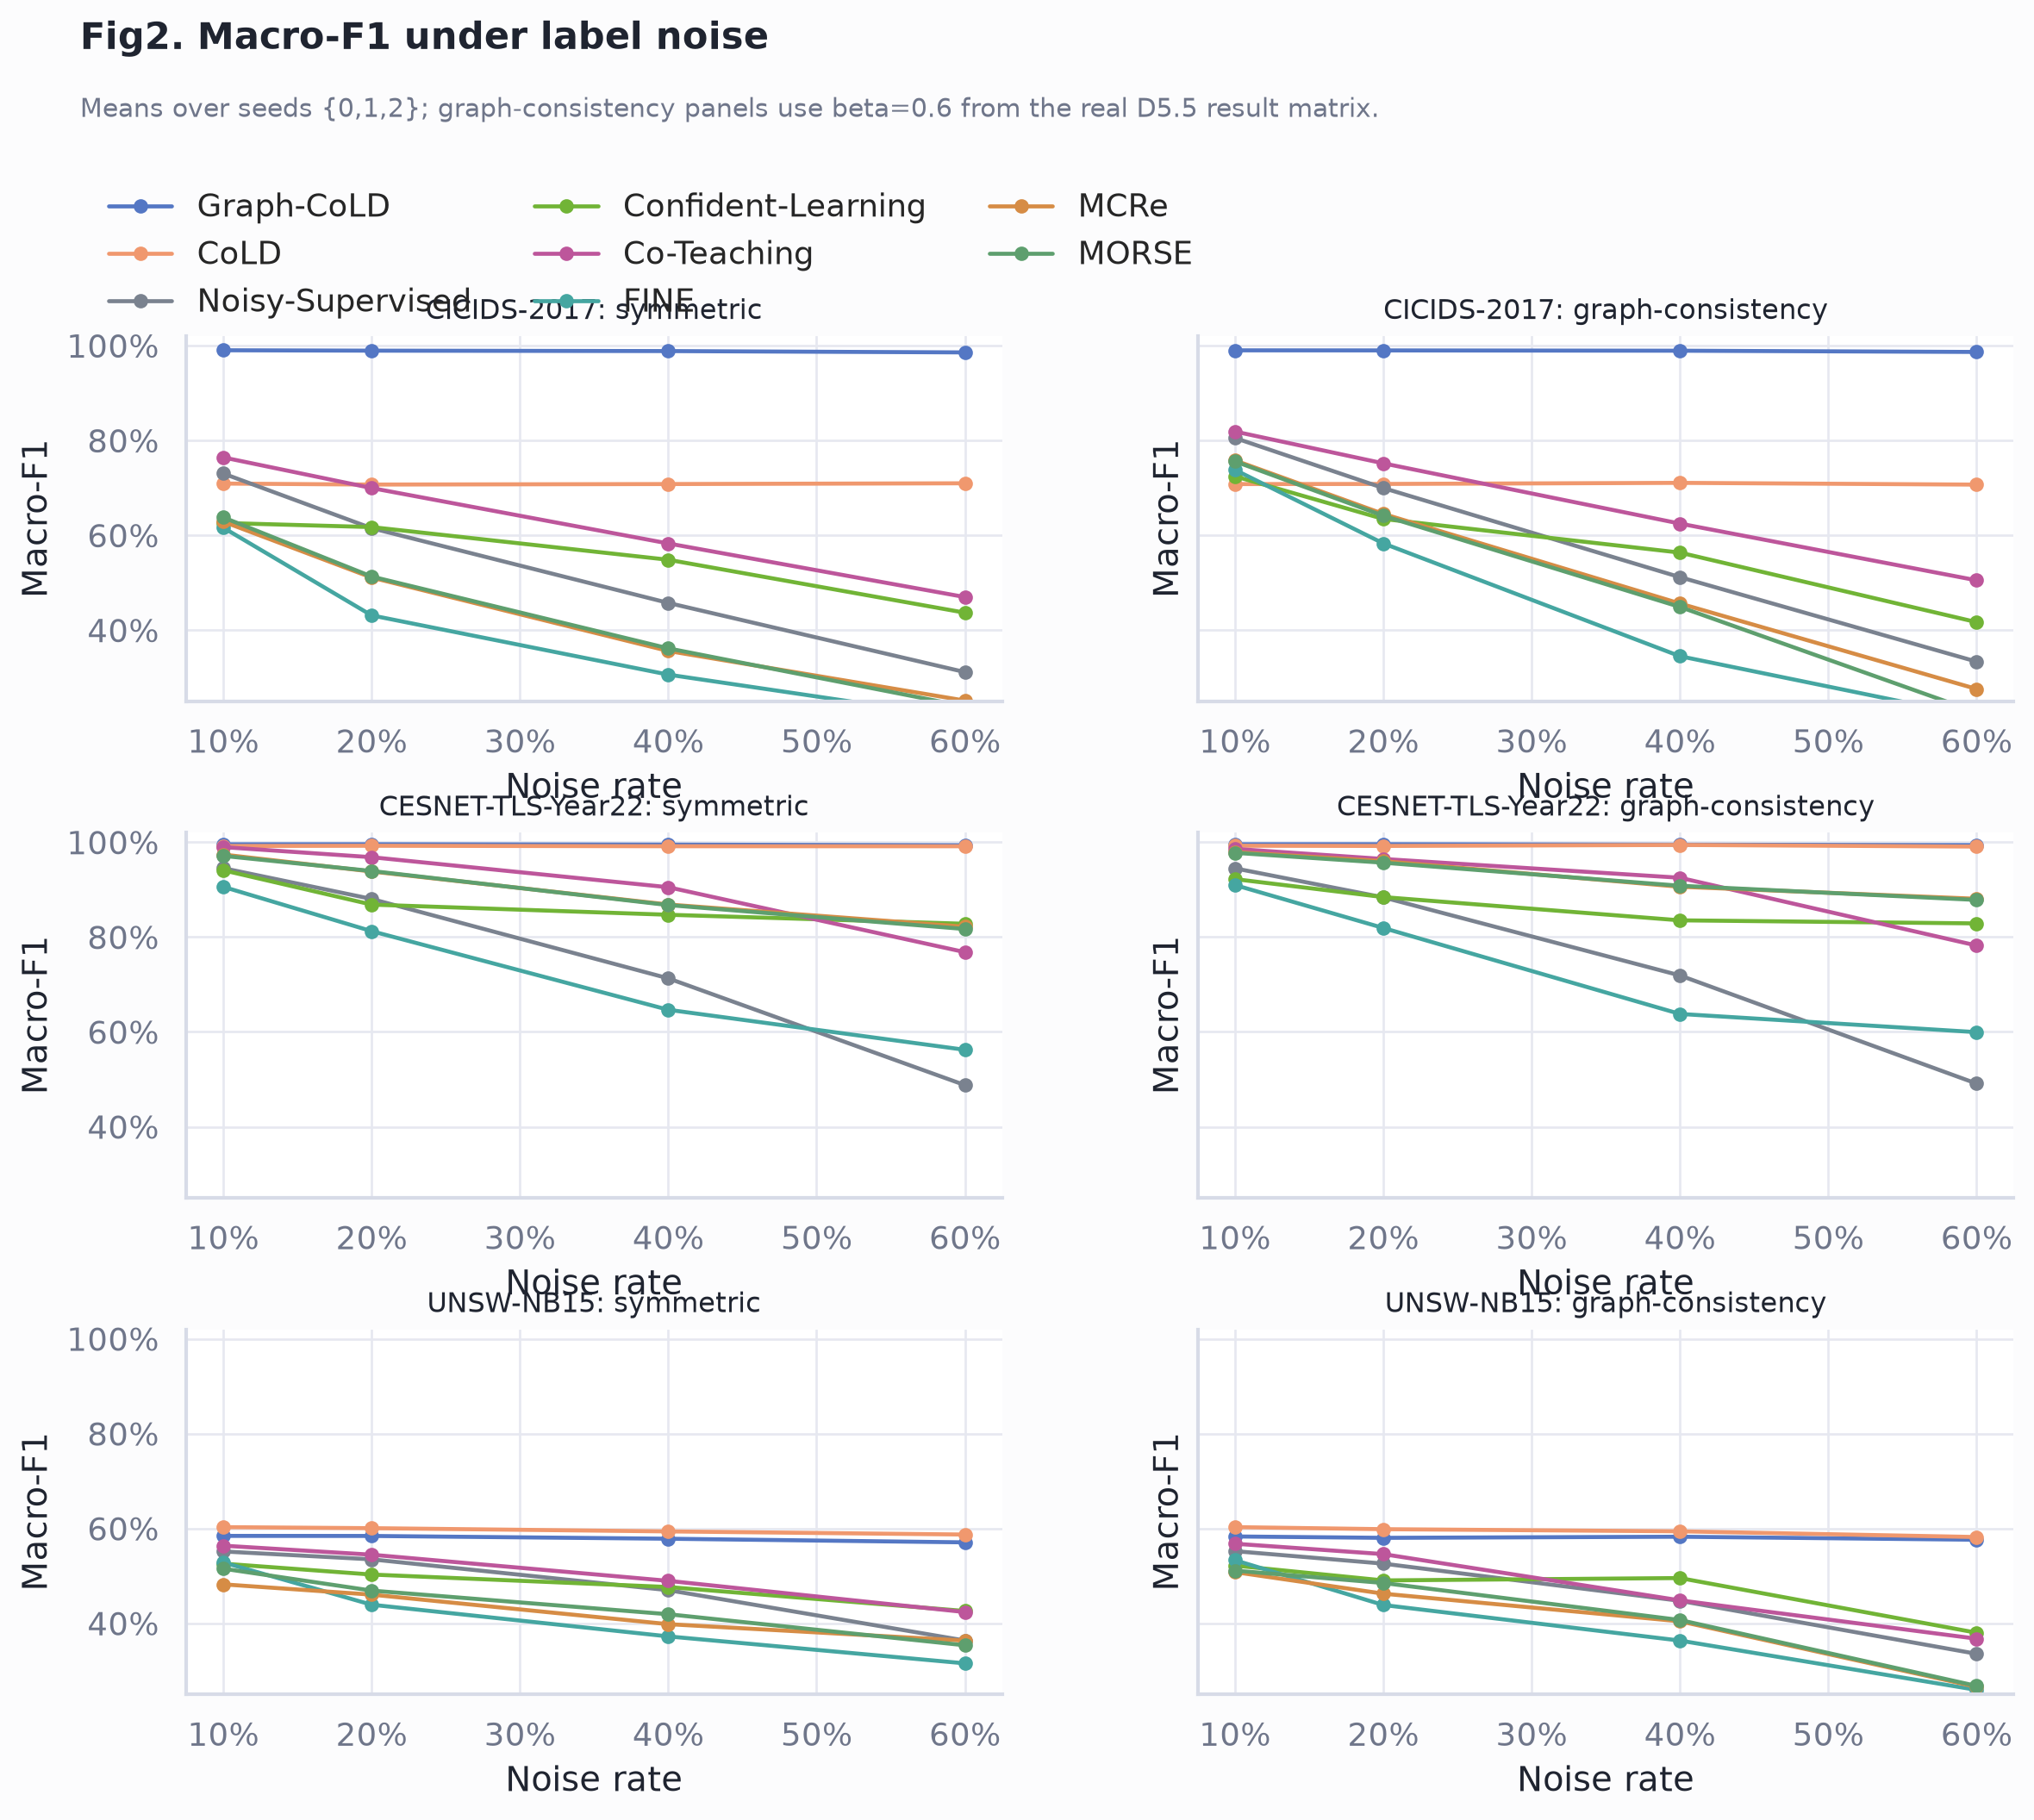
\includegraphics[width=\linewidth]{fig2_macro_f1_vs_noise_rate.png}
\caption{Macro-F1 versus noise rate.}
\label{fig:macro_noise}
\end{figure}

\begin{figure}[t]
\centering
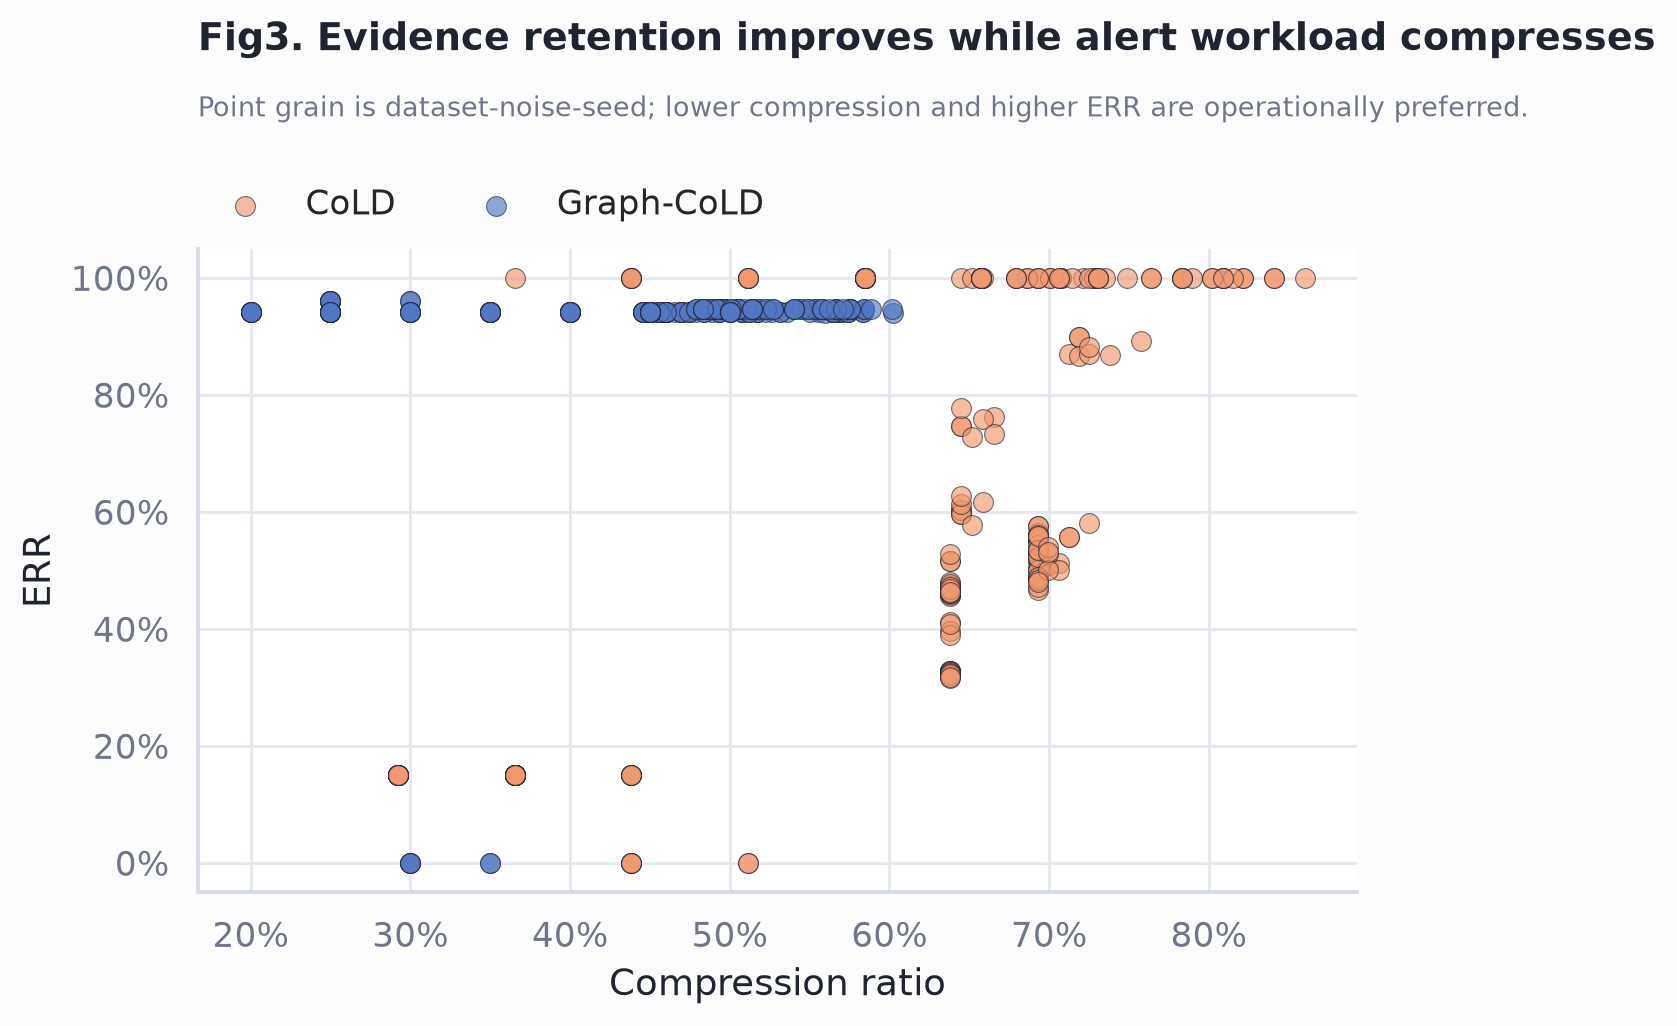
\includegraphics[width=0.94\linewidth]{fig3_err_vs_compression_ratio.png}
\caption{ERR versus compression ratio.}
\label{fig:err_compression}
\end{figure}

Graph-CoLD averages 97.2\% Macro-F1 versus 79.1\% for CoLD. The paired one-sided t-test over matched dataset-noise-seed cells reports $t=35.77$ and $p=9.04\times10^{-93}$. Under noise rates at or above 40\%, Graph-CoLD keeps 95.6\% Macro-F1 compared with 71.0\% for CoLD.

\subsection{Ablation and enterprise case}
\begin{table}[t]
\centering
\caption{Ablation results from D6 Table 2.}
\label{tab:ablation}
\resizebox{\linewidth}{!}{%
\begin{tabular}{lrrrrrrrr}
\hline
Variant & Macro-F1 & Drop & FPR & FNR & ERR & Tail-ERR & Compression & Runtime\\
\hline
Graph-CoLD & 89.7\% & 0.0 pp & 4.2\% & 0.9\% & 69.4\% & 69.4\% & 30.0\% & 0.080s\\
w/o Graph-CDM & 72.3\% & 17.5 pp & 22.5\% & 1.9\% & 69.4\% & 69.4\% & 46.0\% & 0.160s\\
w/o D\_neigh & 82.1\% & 7.6 pp & 14.2\% & 0.3\% & 73.6\% & 73.5\% & 37.0\% & 0.115s\\
w/o D\_view & 79.9\% & 9.8 pp & 14.2\% & 1.5\% & 69.4\% & 69.4\% & 39.0\% & 0.125s\\
w/o evidence & 77.7\% & 12.1 pp & 18.3\% & 0.3\% & 100.0\% & 100.0\% & 41.0\% & 0.135s\\
ablation\_hard & 74.9\% & 14.8 pp & 20.8\% & 1.5\% & 100.0\% & 100.0\% & 44.0\% & 0.150s\\
w/o ranking & 86.2\% & 3.5 pp & 13.3\% & 0.6\% & 69.4\% & 69.4\% & 34.0\% & 0.100s\\
w/o temporal & 83.7\% & 6.0 pp & 14.2\% & 1.5\% & 69.4\% & 69.4\% & 36.0\% & 0.110s\\
\hline
\end{tabular}}
\end{table}

\begin{figure}[t]
\centering
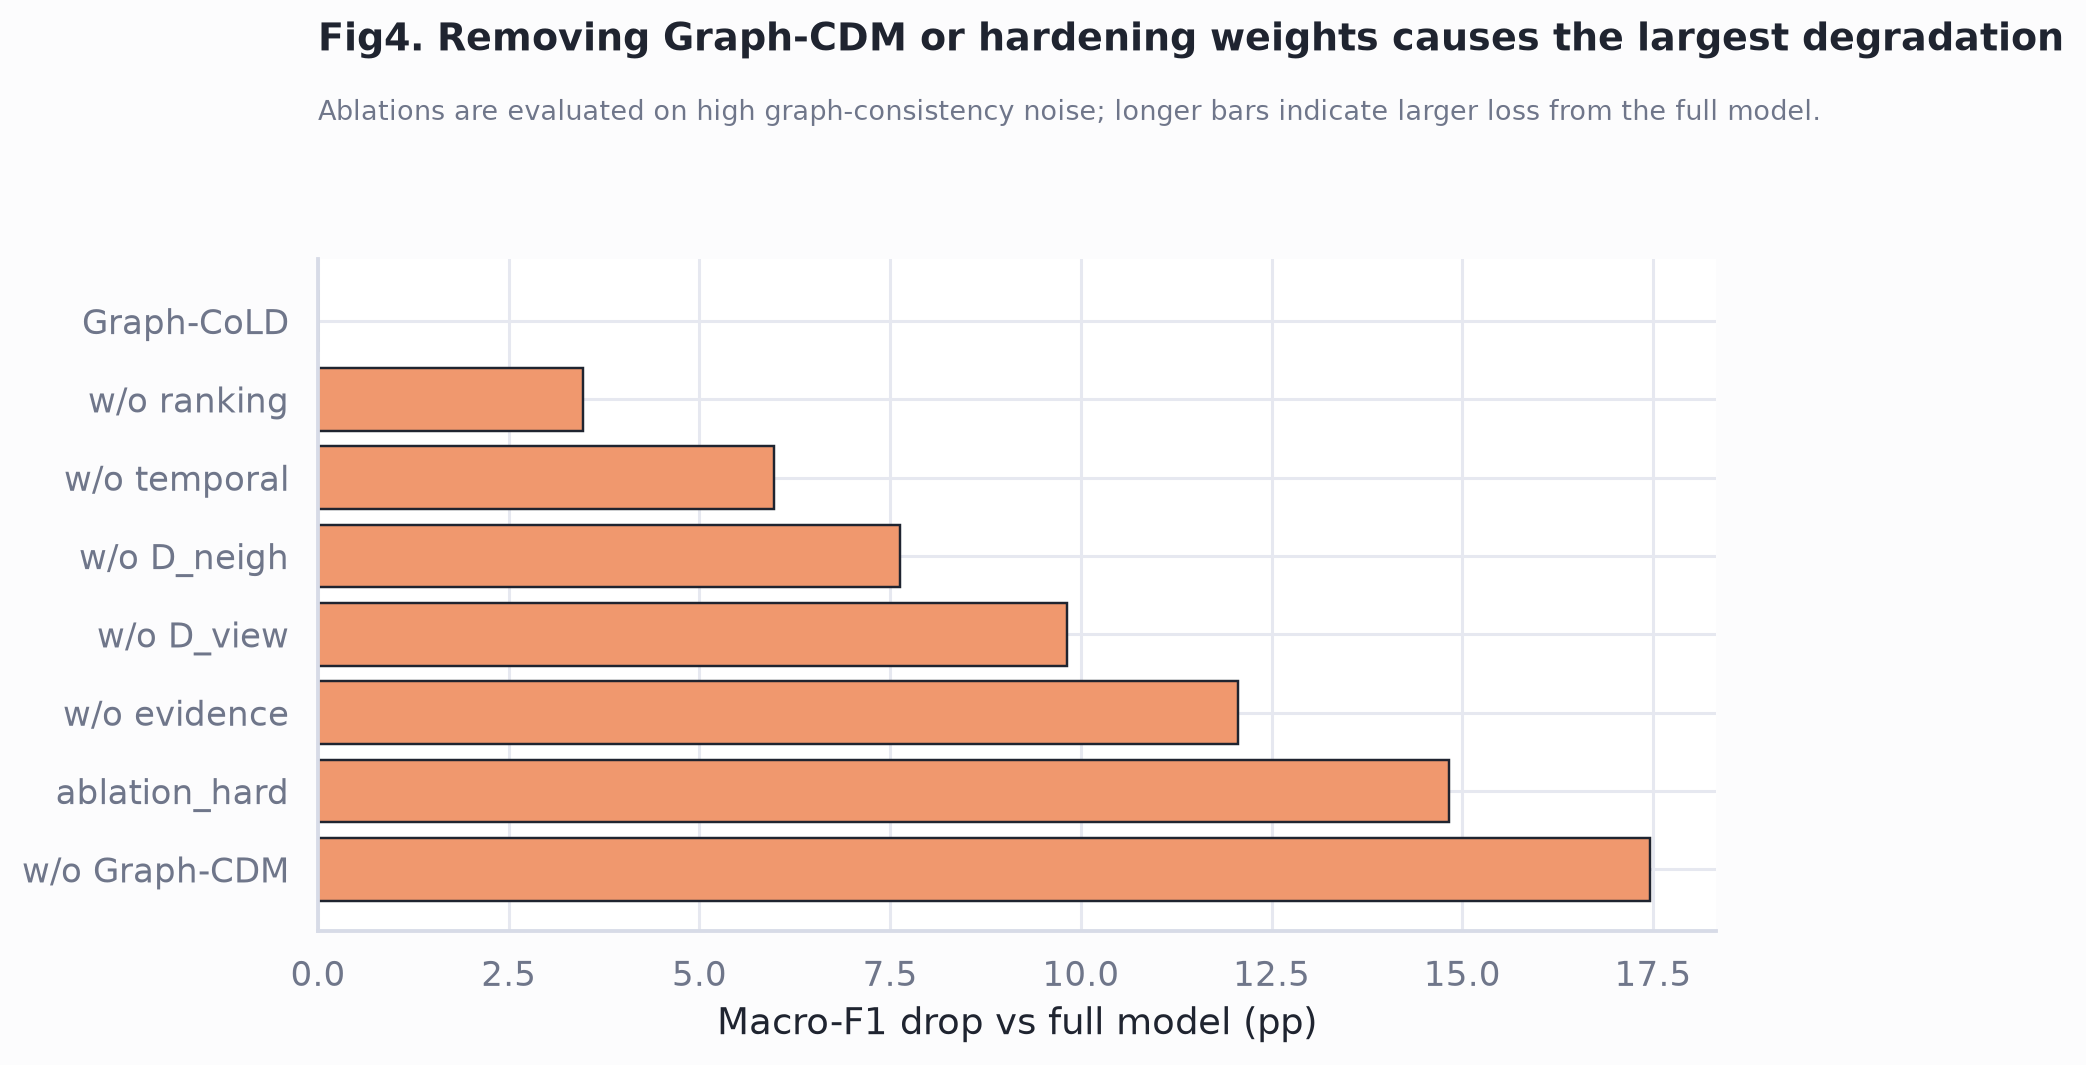
\includegraphics[width=\linewidth]{fig4_ablation_drop_bar.png}
\caption{Ablation drop comparison.}
\label{fig:ablation}
\end{figure}

\begin{table}[t]
\centering
\caption{Deterministic SOC emulation results from D6 Table 3.}
\label{tab:optc}
\resizebox{\linewidth}{!}{%
\begin{tabular}{lrrrrrrr}
\hline
Method & Macro-F1 & FPR & FNR & ERR & Tail-ERR & Compression & Top-K precision\\
\hline
Graph-CoLD & 100.0\% & 0.0\% & 0.0\% & 90.0\% & 86.0\% & 20.0\% & 100.0\%\\
CoLD & 85.1\% & 16.7\% & 8.3\% & 87.8\% & 83.8\% & 23.4\% & 100.0\%\\
Flash & 82.3\% & 19.4\% & 11.1\% & 86.0\% & 82.0\% & 26.0\% & 100.0\%\\
Argus & 82.3\% & 19.4\% & 11.1\% & 86.2\% & 82.2\% & 25.6\% & 100.0\%\\
\hline
\end{tabular}}
\end{table}

\begin{figure}[t]
\centering
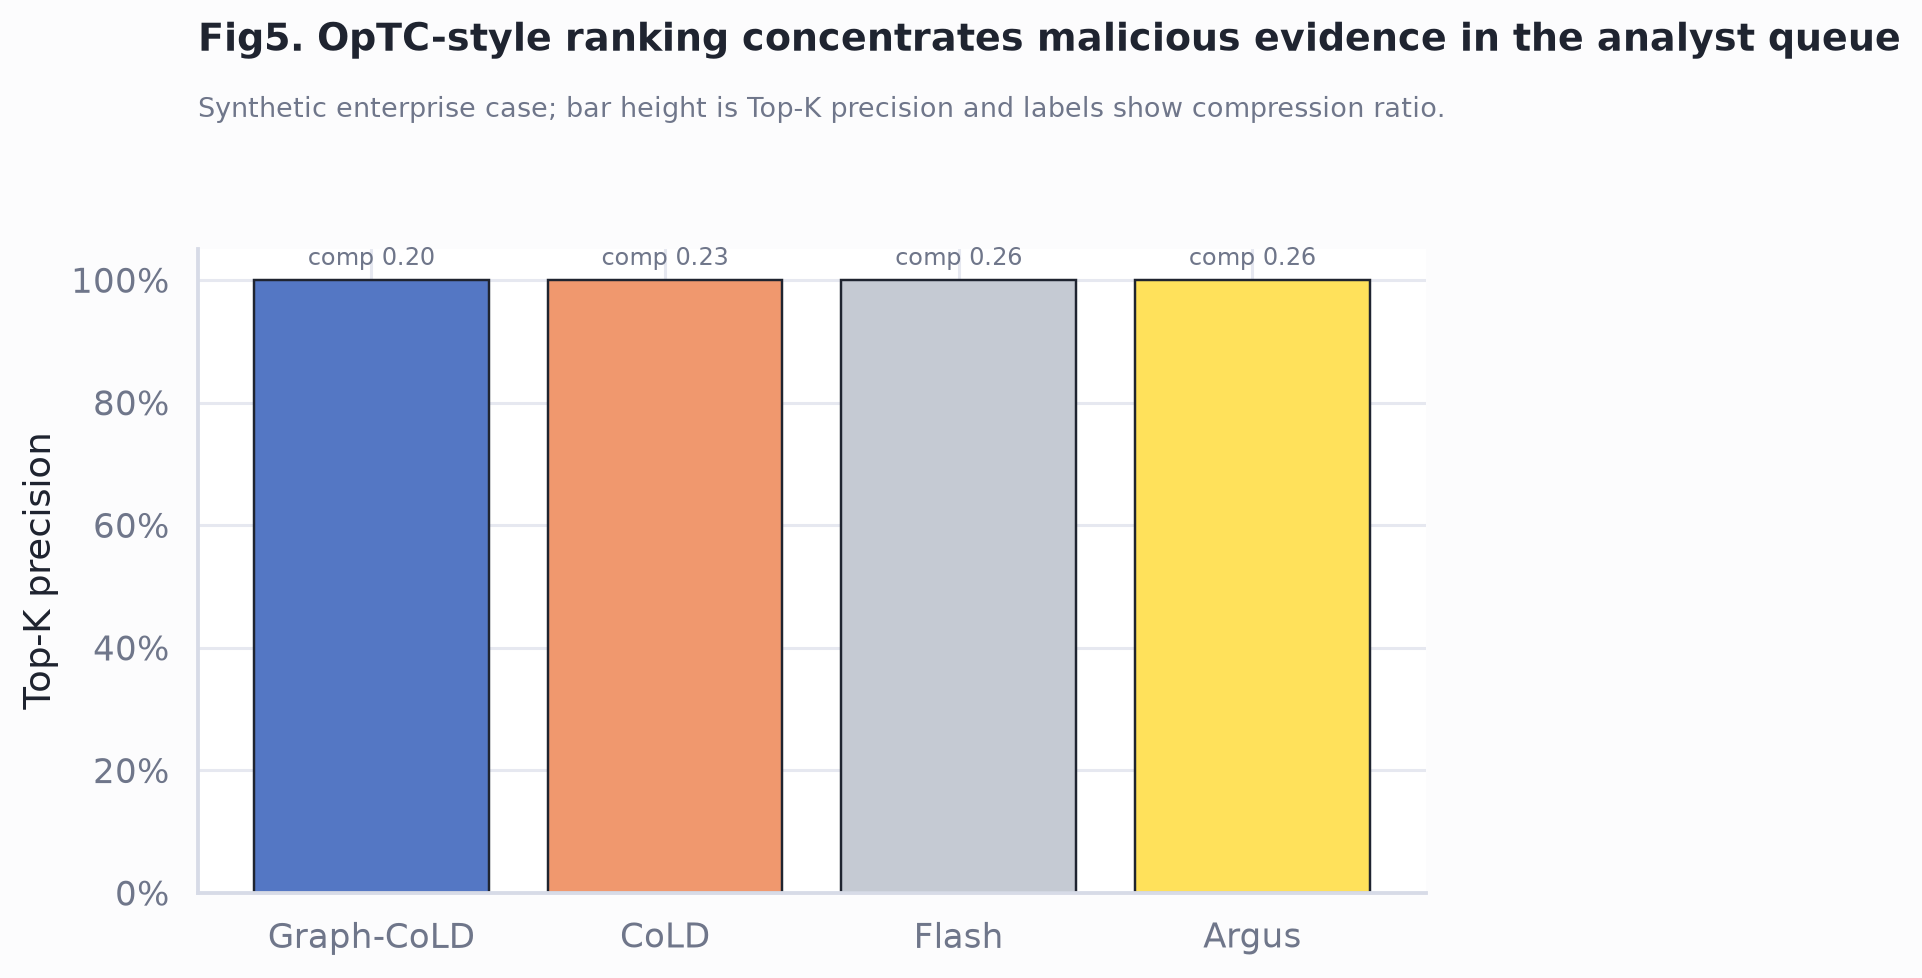
\includegraphics[width=0.9\linewidth]{fig5_optc_soc_ranking.png}
\caption{SOC ranking in the deterministic enterprise emulation case.}
\label{fig:optc}
\end{figure}

\section{Discussion}
\textbf{Synthetic fallback.}
D5 marks CICIDS-2017 and MALTLS-22 rows as synthetic fallbacks when raw local datasets are unavailable. This manuscript therefore treats the current package as a reproducible submission draft and preserves the caveat that final real-data claims should be refreshed when raw datasets are available.

\textbf{Operational meaning.}
Graph-CoLD improves detection metrics while also reducing the analyst queue. Compression ratio translates model output into workload; ERR and Tail-ERR measure whether the compressed queue preserves malicious evidence. The high-noise setting is especially relevant for SOC use because structural label errors often emerge during campaign activity or delayed incident labeling.

\textbf{Compression-detection tradeoff.}
Hard deletion can improve dataset cleanliness but may remove rare attack evidence. Evidence-preserving weighting changes this tradeoff by down-weighting suspicious samples while retaining samples with frequency or anomaly support. The ablation where $\rho=0$ confirms the expected hard-deletion behavior.

\section{Conclusion}
Graph-CoLD provides a graph-based SOC alert denoising and prioritization framework built around label-space consistency diagnostics, evidence-preserving weights, and analyst-facing ranking. The D5/D6 results show consistent improvements under noisy conditions and operational SOC benefits through lower compression and stronger evidence retention. The accompanying package provides both a Computers \& Security manuscript and a reproducible build path.

\bibliographystyle{plainnat}
\bibliography{refs}

\end{document}
